\documentclass[lang=cn,10pt,cnfont=NotoCJK]{../simplebook}

\usepackage{hologo}
\usepackage{listings}

\renewcommand{\ttdefault}{cmtt}
\lstdefinestyle{mystyle}{
basicstyle=%
    \ttfamily
    \lst@ifdisplaystyle\small\fi
}

\lstset{basicstyle=\ttfamily,style=mystyle,breaklines=true}

\definecolor{lightgrey}{rgb}{0.9,0.9,0.9}
\definecolor{frenchplum}{RGB}{190,20,83}
\lstset{language=[LaTeX]TeX,
texcsstyle=*\color{winered},
numbers=none,
mathescape=false,
breaklines=true,
keywordstyle=\color{winered},
commentstyle=\color{gray},
emph={simplepaper,fontenc,fontspec,cnfont,xeCJK,citestyle,FiraMono,xunicode,figure,fig,image,img,table,itemize,enumerate,ctex,microtype,description,times,booktabs,tabular,PDFLaTeX,XeLaTeX,type1cm,BibTeX,color,mode,lang,amsthm,tcolorbox,titlestyle,cite,ctex,listings,base,math,scheme,toc,esint,chinesefont,amsmath,bibstyle,natbib,pgfornament,addbibresource,printbibliography},
emphstyle={\color{frenchplum}},
morekeywords={DeclareSymbolFont,SetSymbolFont,toprule,midrule,bottomrule,institute,version,includegraphics,setmainfont,setsansfont,setmonofont ,setCJKmainfont,setCJKsansfont,setCJKmonofont,RequirePackage,figref,tabref,email,maketitle,keywords,definecolor,bottominfo,logo,cover,subtitle,appendix,chapter,section,hypersetup,mainmatter,frontmatter,tableofcontents,heiti,kaishu,lstset,pagecolor,zhnumber,part,equote,bioinfo,datechange,listofchange,lvert,lastpage,songti,heiti,fangsong,setCJKfamilyfont,textbf,thmcnt,colorlet,usesamecnt},
frame=single,
tabsize=2,
rulecolor=\color{ecolor},
framerule=0.2pt,
columns=flexible,
% backgroundcolor=\color{lightgrey}
}
\renewcommand\ttdefault{lmtt}

\title{SimpleBook 书籍模板}
\subtitle{基于 ElegantBook 的\LaTeX{}模板}

\author{Fenglielie}
% \institute{None}
\date{2024-03-22}
\bottominfo{}
\cover{legao.jpg}
%\logo{logo-blue.png}

\setcounter{tocdepth}{2}

\RequirePackage[backend=biber,citestyle=numeric-comp,bibstyle=numeric]{biblatex}
\addbibresource[location=local]{reference.bib}

\begin{document}

\maketitle

\frontmatter

\chapter*{前言}

SimpleBook是基于\href{https://github.com/ElegantLaTeX/ElegantBook}{ElegantBook}修改的笔记模板,
ElegantBook是一个著名的开源书籍模板,但是原作者在2023年1月1日已经停止更新,因此选择以它的最终版为基础,
对其进行整理和简化:删除了大部分花哨的美化配置,清理了ElegantBook出于版本兼容性保留的代码。

项目部署在Github: \href{https://github.com/fenglielie/simplebook/}{https://github.com/fenglielie/simplebook/}。


\tableofcontents

\mainmatter


\chapter{配置说明}

SimpleBook支持两种编译方式:\hologo{pdfLaTeX} 和 \hologo{XeLaTeX}。
支持中文和英文两种模式:英文模式下用任意编译方式均可,中文模式下必须使用 \hologo{XeLaTeX}。
在使用SimpleBook文档类时,有如下主要选项:

\begin{enumerate}
    \item 语言:中文cn(默认),英文en;
    \item 颜色:决定主题色,包括blue(默认)和black;
    \item 中文字体:决定中文字体,包括ctex的几个默认方案,以及开源的方正字体,思源字体方案,见下文。
\end{enumerate}


\begin{remark}
    文档类的选项既可以使用完整的键值对形式,例如\lstinline{device=normal},
    也可以直接使用选项名\lstinline{normal},并且多个选项可以连续设置,并且任意顺序均可。
\end{remark}


\section{语言}
本模板内含两套基础语言环境 \lstinline{lang=cn}、\lstinline{lang=en},默认中文。改变语言环境会改变图表标题的引导词(图,表),文章结构词(比如目录,参考文献等),以及定理环境中的引导词(比如定理,引理等)。不同语言模式的启用如下:
\begin{lstlisting}
\documentclass[cn]{simplebook}
\documentclass[lang=cn]{simplebook}
\end{lstlisting}


\section{颜色}

本模板默认主题颜色为蓝绿色调\lstinline{blue},可以改成\lstinline{color=black}即全为黑色。
如果需要自定义颜色的话请选择 \lstinline{nocolor} 选项或者使用 \lstinline{color=nocolor},
然后在导言区定义 ecolor、main、second、third 颜色,具体方法如下:
\begin{lstlisting}[tabsize=4]
\definecolor{ecolor}{RGB}{0,0,0}
\definecolor{main}{RGB}{70,70,70}
\definecolor{second}{RGB}{115,45,2}
\definecolor{third}{RGB}{0,80,80}
\end{lstlisting}


\section{中文字体}

模板支持不同的中文字体配置,通过\lstinline{cnfont=XXX}设置,默认值为\lstinline{cnfont=auto},支持如下的值:
\begin{enumerate}
    \item 兼容ctex宏包关于中文字体的部分选项:
          \begin{enumerate}
              \item \lstinline{cnfont=auto},令ctex根据系统自动选择字体方案
              \item \lstinline{cnfont=windows},令ctex选择windows字体方案(Windows默认)(传递\lstinline{fontset=windows}参数)
              \item \lstinline{cnfont=fandol},令ctex选择fandol字体方案(Linux默认)(传递\lstinline{fontset=fandol}参数)
              \item \lstinline{cnfont=none},禁止ctex的字体配置(传递\lstinline{fontset=none}参数)
          \end{enumerate}
    \item 开源中文字体选项:(向ctex传递\lstinline{fontset=none}参数并自行配置)
          \begin{enumerate}
              \item \lstinline{cnfont=FZ},方正字体(仅使用四个开源字体)
                    \begin{enumerate}
                        \item 方正书宋 FZSSK.TTF,FZShuSong-Z01
                        \item 方正黑体 FZHTK.TTF,FZHei-B01
                        \item 方正楷体 FZKTK.TTF,FZKai-Z03
                        \item 方正仿宋 FZFSK.TTF,FZFangSong-Z02
                    \end{enumerate}
              \item \lstinline{cnfont=NotoCJK},Noto CJK 思源字体(SC简体中文版本)
                    \begin{enumerate}
                        \item 思源宋体 Noto Serif CJK SC
                        \item 思源黑体 Noto Sans CJK SC
                        \item 思源等宽字体 Noto Sans Mono CJK SC
                    \end{enumerate}
              \item \lstinline{cnfont=SourceHan},Source Han 思源字体(SC简体中文版本)
                    \begin{enumerate}
                        \item 思源宋体 Source Han Serif SC
                        \item 思源黑体 Source Han Sans SC
                    \end{enumerate}
          \end{enumerate}
\end{enumerate}

\begin{remark}
    由于思源字体只有思源宋体和思源黑体,缺少通常的楷体(作为宋体的斜体)和仿宋,因此需要使用方正楷体和方正仿宋作为补充,
    换言之,这几个方案都需要安装四个方正开源字体。
\end{remark}

\begin{remark}
    各个在线编译平台(例如Overleaf)支持的中文字体并不统一:
    由于部署在Linux服务器上,fandol字体是最可能可用的,思源字体和windows的字体有时也可用,通常都不含方正开源字体。
\end{remark}

如果选择\lstinline{cnfont=none},还可以自行进行配置,参考代码如下:
\begin{lstlisting}[frame=single]
\setCJKmainfont{FZShuSong-Z01}[BoldFont={FZHei-B01},ItalicFont={FZKai-Z03}]
\setCJKsansfont{FZKai-Z03}[BoldFont={FZHei-B01}]
\setCJKmonofont{FZFangSong-Z02}[BoldFont={FZHei-B01}]

\setCJKfamilyfont{zhsong}{FZShuSong-Z01}
\setCJKfamilyfont{zhhei}{FZHei-B01}
\setCJKfamilyfont{zhkai}{FZKai-Z03}[BoldFont={FZHei-B01}]
\setCJKfamilyfont{zhfs}{FZFangSong-Z02}[BoldFont={FZHei-B01}]

\newcommand*{\songti}{\CJKfamily{zhsong}}
\newcommand*{\heiti}{\CJKfamily{zhhei}}
\newcommand*{\kaishu}{\CJKfamily{zhkai}}
\newcommand*{\fangsong}{\CJKfamily{zhfs}}
\end{lstlisting}

\section{封面信息}

目前模板的封面支持很多元素,包括 \lstinline{\title} 在内的所有封面元素都可为空。

\begin{itemize}
    \item \textbf{标题 (Title)}: \lstinline|\title|
    \item \textbf{副标题 (Subtitle)}: \lstinline|\subtitle|
    \item \textbf{作者 (Author)}: \lstinline|\author|
    \item \textbf{机构 (Institute)}: \lstinline|\institute|
    \item \textbf{日期 (Date)}: \lstinline|\date|
    \item \textbf{底部信息 (Bottom Info)}: \lstinline|\bottominfo|
    \item \textbf{封面图 (Cover)}: \lstinline|\cover|
    \item \textbf{徽标 (Logo)}: \lstinline|\logo|
\end{itemize}

封面图片必须\textbf{严格}用尺寸$1280 \times 1024$的图片进行替换
\begin{lstlisting}
\cover{demo.jpg}
\end{lstlisting}
封面中间位置的色块的颜色可以使用下面命令进行修改:
\begin{lstlisting}
\definecolor{customcolor}{RGB}{32,178,170}
\colorlet{coverlinecolor}{customcolor}
\end{lstlisting}
封面右下角可以加入Logo,Logo图片要求尺寸比例为1:1,可以省略Logo
\begin{lstlisting}
\logo{demo.jpg}
\end{lstlisting}


\section{参考文献}


原本的ElegantBook模板包括了参考文献的部分:使用Biblatex宏包,并支持通过参数传递样式。
但是出于个人需求的原因,将这部分完全移除,在需要参考文献时自行进行配置。

传统的Bibtex的基本用法如下:
\begin{enumerate}
    \item 导言区指定样式,例如\lstinline|\bibliographystyle{plain}|;
    \item 在显示参考文献列表的位置使用\lstinline|\bibliography{reference}|,这里假设参考文献文件为reference.bib。
\end{enumerate}
示例如下:
\begin{lstlisting}[frame=single]
\documentclass{article}
\bibliographystyle{plain}

\begin{document}

According to Einstein's theory of relativity \cite{einstein1905}...

\bibliography{reference} % reference.bib

\end{document}
\end{lstlisting}

现代的Biblatex的基本用法如下:
\begin{enumerate}
    \item 在导言区导入 biblatex 宏包,可以指定样式和后端等;
    \item 在导言区加载参考文献文件,例如\lstinline|\addbibresource[location=local]{reference.bib}|,这里假设参考文献文件为reference.bib
    \item 在显示参考文献列表的位置使用\lstinline|\printbibliography|
\end{enumerate}
示例如下:
\begin{lstlisting}[frame=single]
\documentclass{article}
\usepackage[style=authoryear]{biblatex}
\addbibresource{reference.bib} % reference.bib

\begin{document}

According to Einstein's theory of relativity \parencite{einstein1905}...

\printbibliography[title={References}]

\end{document}
\end{lstlisting}


\section{数学环境}

本模板支持常见的数学定理环境

\begin{itemize}
    \item \textit{定理类环境},包含标题和内容两部分,全部定理类环境自动以章节为单位编号,计数器相互独立。根据样式的不同可以分为 2 种
          \begin{itemize}
              \item \textcolor{main}{\textbf{definition(定义)}} 环境;
              \item \textcolor{second}{\textbf{theorem(定理)、lemma(引理)、corollary(推论)、proposition(命题)}} 环境;
          \end{itemize}
    \item \textit{示例与题目},有 \textbf{\color{main}{example(例)}、\color{main}{problem(题目)}、\color{main}{exercise(练习)}} 环境,自动以章节为单位编号。
    \item \textit{解答与笔记},有 \textbf{\color{third}{note(笔记)}、\color{third}{remark(注)}、\color{third}{solution(解)}} 环境,无编号。
\end{itemize}
其中定理类环境均有带星号的版本:\textcolor{main}{\textbf{definition*}}、\textcolor{second}{\textbf{theorem*}}、\textcolor{second}{\textbf{lemma*}}、\textcolor{second}{\textbf{corollary*}}、\textcolor{second}{\textbf{proposition*}},带星号的定理类环境不会编号。
除此之外,还有默认可以使用的\textbf{\color{third}{proof(证明)}}环境。

定理类环境的使用例如
\begin{lstlisting}
\begin{theorem}[theorem name]\label{thm:label}
  这是一个有名字和标签的定理。可以用 \ref{thm:label} 来引用这个定理。
\end{theorem}

\begin{theorem}[theorem name]
  这是一个有名字的定理。
\end{theorem}
\end{lstlisting}

其他三种环境没有选项,可以直接使用,比如 \lstinline{example} 环境的使用方法与效果:
\begin{lstlisting}
\begin{example}
   This is the content of example environment.
\end{example}
\end{lstlisting}



\begin{remark}
    原ElegantBook对数学定理环境支持fancy和simple两种模式,但是个人觉得fancy模式下的彩色盒子过于花哨,因此直接删除。
\end{remark}


\chapter{写作示例}

\begin{theorem}[Fubini 定理]\label{thm:fubi}
    若 $f(x,y)$ 是 $\mathcal{R}^p\times\mathcal{R}^q$ 上的非负可测函数,
    则对几乎处处的 $x\in \mathcal{R}^p$,$f(x,y)$ 作为 $y$ 的函数是 $\mathcal{R}^q$ 上的非负可测函数,
    $g(x)=\int_{\mathcal{R}^q}f(x,y) dy$ 是 $\mathcal{R}^p$ 上的非负可测函数。并且
    \begin{equation}\label{eq:461}
        \int_{\mathcal{R}^p\times\mathcal{R}^q} f(x,y) dxdy=\int_{\mathcal{R}^p}\left(\int_{\mathcal{R}^q}f(x,y)dy\right)dx.
    \end{equation}
\end{theorem}


\begin{theorem}
    对于Burgers方程,假设给定光滑的初值$u_0(x)$,并且存在某些点满足$u_0'(x) < 0$,
    那么准确解在$T_b$时刻特征线首次相交,解出现无穷斜率(间断,激波)。
    \[
        T_b = \frac{-1}{\min u_0'(x)}
    \]
\end{theorem}
\begin{proof}
    证明分成两部分:首先证明在$T_b$时刻特征线首次相交,然后证明在$T_b$时刻会出现无穷斜率,证明细节略。
\end{proof}


\begin{lemma}[Harten引理]
    若差分格式可以表述为如下形式
    \[
        v_j^{n+1} = v_j^n - C_{j-1/2}(v_j^n - v_{j-1}^n) + D_{j+1/2}(v_{j+1}^n - v_j^n)
    \]
    且处处成立
    \[
        C_{j+1/2} \ge 0, D_{j+1/2} \ge 0, C_{j+1/2} + D_{j+1/2} \le 1, \forall j
    \]
    则它是TVD格式。
\end{lemma}

\begin{proposition}
    下面两个结论等价:
    \begin{enumerate}
        \item 存在常数$\delta >0$,使得$A$的所有特征值$\lambda$都满足$\Re\, \lambda \ge \delta$;(即抛物的定义)
        \item 存在常数$\delta >0$,使得$A + A^* \ge \delta I$。
    \end{enumerate}
\end{proposition}

\begin{corollary}
    单调格式一定是TVD格式,TVD格式一定是单调保持格式,反之不成立。
    限于线性差分格式的范畴,单调格式、TVD格式和单调保持格式这三个概念是彼此等价的。
\end{corollary}

\begin{definition}[守恒型格式]
    称差分格式为守恒型格式,若它可以表述为如下形式
    \begin{equation}
        v_{j}^{n+1} = v_j^n - \frac{\Delta t}{\Delta x}\left(
        \hat{f}_{j+1/2}^n - \hat{f}_{j-1/2}^n
        \right) \tag{$*$}
    \end{equation}
    其中$\hat{f}_{j+\frac12}$称为数值流通量,具有表达式$\hat{f}_{j+\frac12} = \hat{f}(v_{j-r},\cdots,v_{j+s})$,
    并且满足
    \begin{enumerate}
        \item 连续性:$\hat{f}$关于每一个变量都是局部Lipschitz连续的
        \item 相容性:$\hat{f}(v,\dots,v) = f(v)$
    \end{enumerate}
\end{definition}


\begin{example}
    Burgers方程$u_t + u u_x = 0$的特征线满足
    \begin{equation}
        \frac{d x}{d t} = f'(u_0(x_0)) = u_0(x_0)
    \end{equation}
    特征线为$x\!-\!t$平面的直线
    \begin{equation}
        x = x_0 + u_0(x_0) t \label{eq:1}
    \end{equation}
\end{example}

下面是图片和表格的示例,其中\figref{fig:1}呈现了一个典型的Burgers方程精确解,
通过求解非线性方程\eqref{eq:1}得到;\tabref{tab:1}呈现了一组数值算法的对比,包括误差和阶数。


\begin{figure}[htbp]
    \centering
    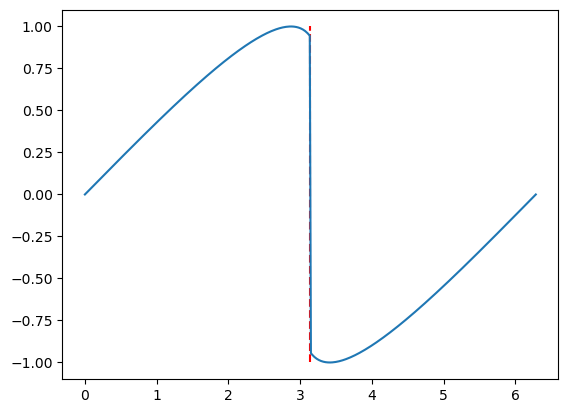
\includegraphics[width=.6\textwidth]{burgers.png}
    \caption{Solution of Burgers' equation}
    \label{fig:1}
\end{figure}

\begin{table}[ht]
    \centering
    \caption{计算结果}\label{tab:1}
    \begin{tabular}{c|c|ccccc}
        \hline
                              &      & N=25     & N=50       & N=100      & N=200      & N=400      \\
        \hline
        \multirow{4}{*}{FTCS} & 误差   & 2.8e-03  & 7.1121e-04 & 1.7821e-04 & 4.4559e-05 & 1.1139e-05 \\
                              & 误差阶数 & -        & 1.97       & 1.99       & 2.00       & 2.00       \\
                              & 时间/s & 0.009449 & 0.009827   & 0.087355   & 0.840438   & 33.303874  \\
        \hline
        \multirow{4}{*}{SVD}  & 误差   & 2.8e-03  & 7.1121e-04 & 1.7847e-04 & 4.4615e-05 & 1.1153e-05 \\
                              & 误差阶数 & -        & 1.97       & 1.99       & 2.00       & 2.00       \\
                              & 时间/s & 0.016365 & 0.010492   & 0.034441   & 0.205993   & 1.431576   \\
        \hline
    \end{tabular}
\end{table}

\begin{problem}
Determine the order of accuracy of the following difference
equations to the partial differential equation
\begin{equation*}
    u_t+au_x=0
\end{equation*}
\begin{equation*}
    v^{n+1}_k=v^{n-1}_k-R\delta_0u^n_k+\frac{R}{6}\delta^2\delta_0u^n_k
\end{equation*}
\end{problem}
\begin{solution}
    截断误差为
    \begin{equation*}
        \begin{aligned}
            T^n_k= & \frac{u^{n+1}_k-u^{n-1}_k}{2\Delta t}+\frac{a}{2\Delta x}(u^n_{k+1}-u^n_{k-1})-\frac{a}{12\Delta x}(u^n_{k+2}-2u^n_{k+1}+2u^n_{k-1}-u^n_{k-2}) \\
            =      & (u_t+\frac{\Delta t^2}{6}u_{ttt}+O(\Delta t^4))|^n_k+a(u_x+\frac{\Delta x^2}{6}u_{xxx}+\frac{\Delta x^4}{120}u_{xxxxx}+O(\Delta x^6))|^n_k     \\
                   & -\frac{a}{12}(2\Delta x^2u_{xxx}+\frac{\Delta x^4}{2}u_{xxxxx}+O(\Delta x^6))|^n_k                                                             \\
            =      & O(\Delta t^2+\Delta x^4)
        \end{aligned}
    \end{equation*}
    关于时间2阶,空间4阶。
\end{solution}

\begin{remark}
    这是remark内容测试。\footfullcite{lubichProjectorsplittingIntegratorDynamical2014}
\end{remark}


\begin{note}
    这是note内容测试。\autocite{kochDynamicalLowRank2007}
\end{note}


多层无序列表效果如下
\begin{itemize}
    \item xxx
    \item xxx
          \begin{itemize}
              \item yyy
              \item yyy
                    \begin{itemize}
                        \item zzz
                        \item zzz
                              \begin{itemize}
                                  \item www
                                  \item www
                              \end{itemize}
                    \end{itemize}
          \end{itemize}
\end{itemize}

多层有序列表效果如下
\begin{enumerate}
    \item xxx
    \item xxx
          \begin{enumerate}
              \item yyy
              \item yyy
                    \begin{enumerate}
                        \item zzz
                        \item zzz
                              \begin{enumerate}
                                  \item www
                                  \item www
                              \end{enumerate}
                    \end{enumerate}
          \end{enumerate}
\end{enumerate}


\nocite{*}

\printbibliography[heading=bibintoc, title={参考文献}]
\appendix

\chapter{基本数学工具}


本附录包括了计量经济学中用到的一些基本数学,我们扼要论述了求和算子的各种性质,研究了线性和某些非线性方程的性质,并复习了比例和百分数。我们还介绍了一些在应用计量经济学中常见的特殊函数,包括二次函数和自然对数,前 4 节只要求基本的代数技巧,第 5 节则对微分学进行了简要回顾;虽然要理解本书的大部分内容,微积分并非必需,但在一些章末附录和第 3 篇某些高深专题中,我们还是用到了微积分。

\section{求和算子与描述统计量}

\textbf{求和算子} 是用以表达多个数求和运算的一个缩略符号,它在统计学和计量经济学分析中扮演着重要作用。如果 $\{x_i: i=1, 2, \ldots, n\}$ 表示 $n$ 个数的一个序列,那么我们就把这 $n$ 个数的和写为:

\begin{equation}
    \sum_{i=1}^n x_i \equiv x_1 + x_2 +\cdots + x_n
\end{equation}


\end{document}
